% Op icon: circular pattern — one solid square (the original) plus ghosted
% copies arranged around a dashed guide circle and centre point.
\documentclass[tikz,border=2mm]{standalone}
\usetikzlibrary{arrows.meta,calc,shapes.geometric}
\begin{document}
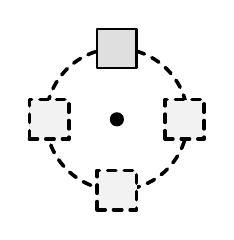
\begin{tikzpicture}[line width=1.3pt, line cap=round, line join=round, >=Stealth, x=1mm,y=1mm]
  \draw[dashed] (0,0) circle (9);
  \fill (0,0) circle (0.9);
  \draw[thick, fill=gray!25] (-2.5,6.5) rectangle (2.5,11.5);
  \draw[dashed, fill=gray!10] (6.1,-2.5) rectangle (11.1,2.5);
  \draw[dashed, fill=gray!10] (-11.1,-2.5) rectangle (-6.1,2.5);
  \draw[dashed, fill=gray!10] (-2.5,-11.5) rectangle (2.5,-6.5);
\end{tikzpicture}
\end{document}
